\lstinputlisting[language=bash,basicstyle=\small]{python_codes/fieldstone_75/keywords}

\begin{center}
Code at \url{https://github.com/cedrict/fieldstone/tree/master/python_codes/fieldstone_75}
\end{center}

\par\noindent\rule{\textwidth}{0.4pt}

%%%%%%%%%%%%%%%%%%%%%%%%%%%%%%%%%%%%%%%%%%%%%%%%%%%%%%%%%%%%%%%%%%%%%%%%%%%%%%%%%%%%%%%%%%%%

\paragraph{The 'Burstedde' benchmark} It is called like this in the ASPECT manual 
but it originates in Dohrmann \& Bochev (2004) \cite{dobo04}. It is carried 
out with $Q_2 \times Q_1$ elements in Stone 17. 

Python file is {\tt stone\_burst.py}

\begin{center}
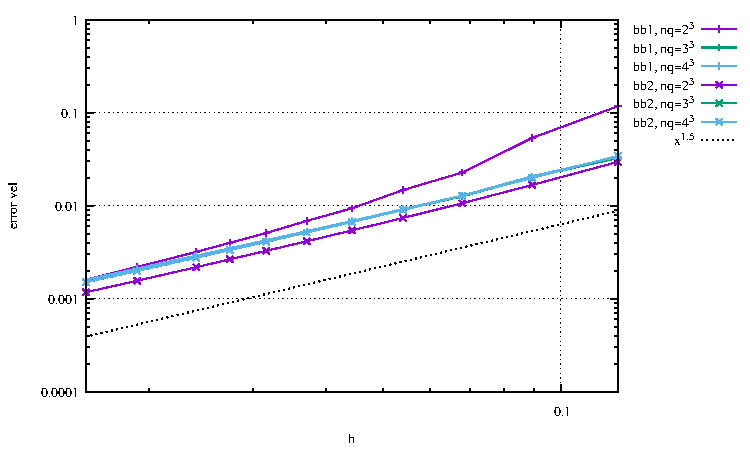
\includegraphics[width=5cm]{python_codes/fieldstone_75/results/burst/errors_v.pdf}
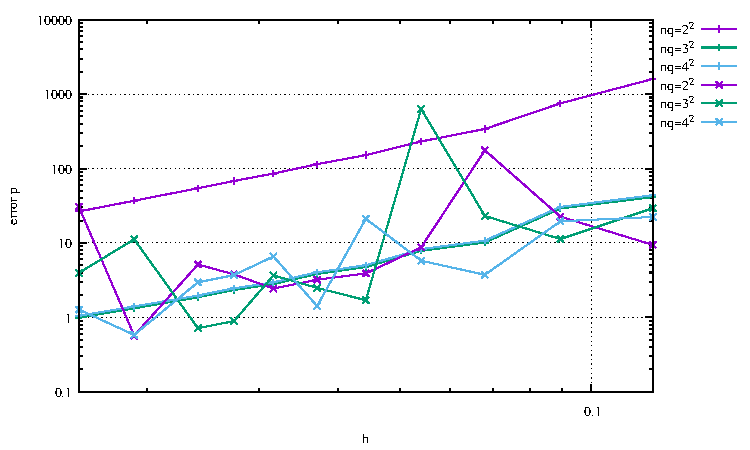
\includegraphics[width=5cm]{python_codes/fieldstone_75/results/burst/errors_p.pdf}
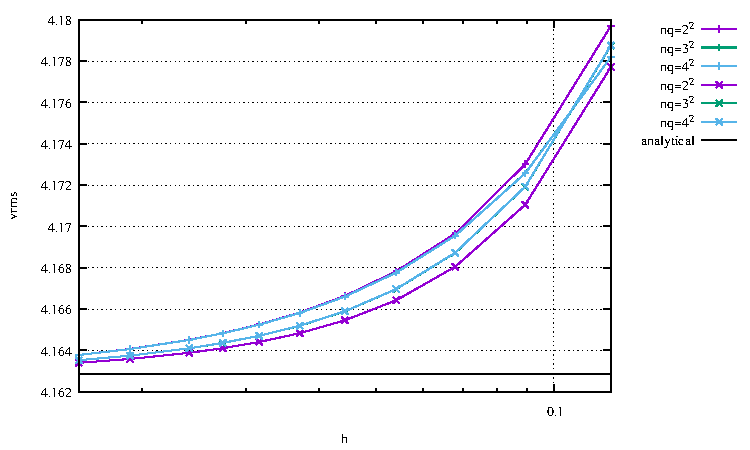
\includegraphics[width=5cm]{python_codes/fieldstone_75/results/burst/vrms.pdf}\\
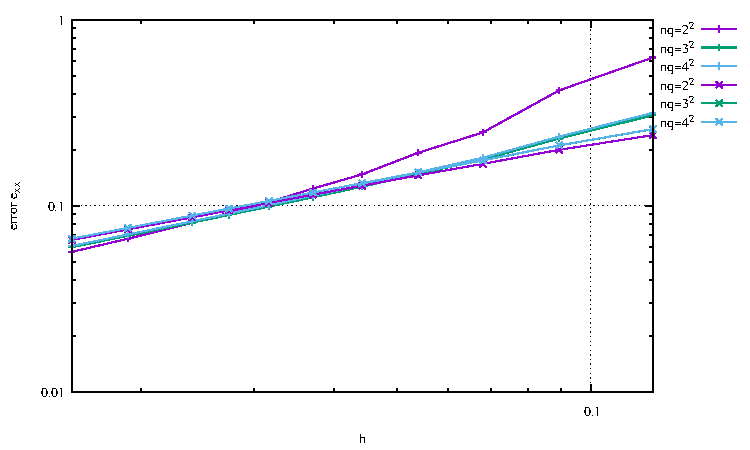
\includegraphics[width=5cm]{python_codes/fieldstone_75/results/burst/errors_exx}
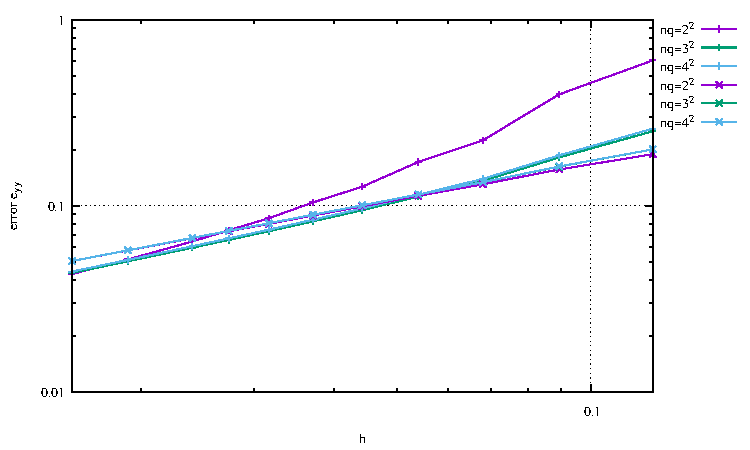
\includegraphics[width=5cm]{python_codes/fieldstone_75/results/burst/errors_eyy}
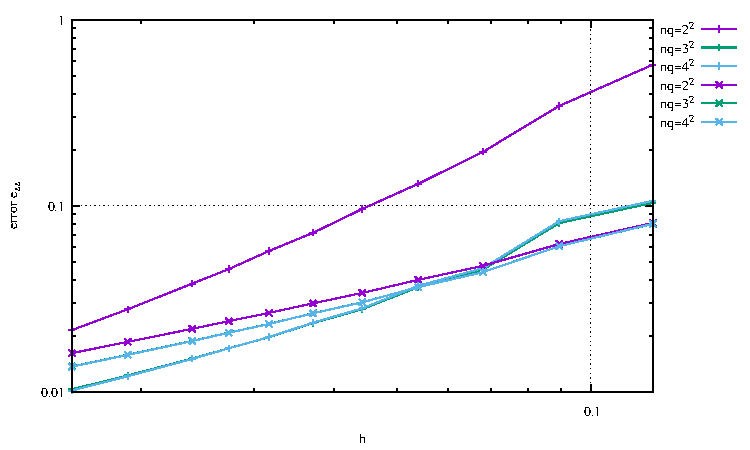
\includegraphics[width=5cm]{python_codes/fieldstone_75/results/burst/errors_ezz}\\
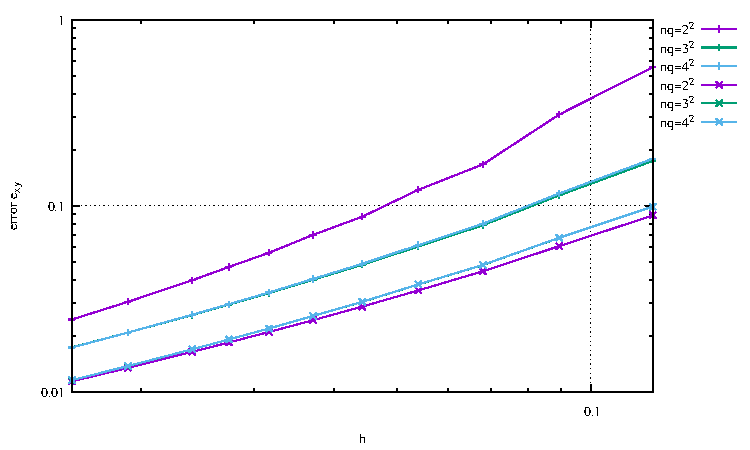
\includegraphics[width=5cm]{python_codes/fieldstone_75/results/burst/errors_exy}
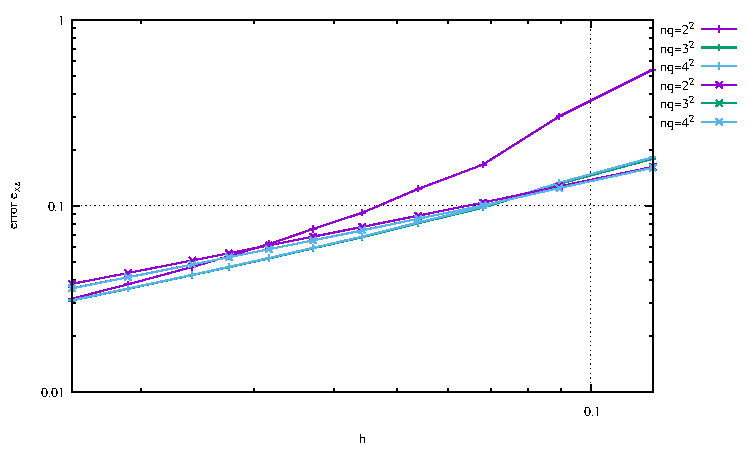
\includegraphics[width=5cm]{python_codes/fieldstone_75/results/burst/errors_exz}
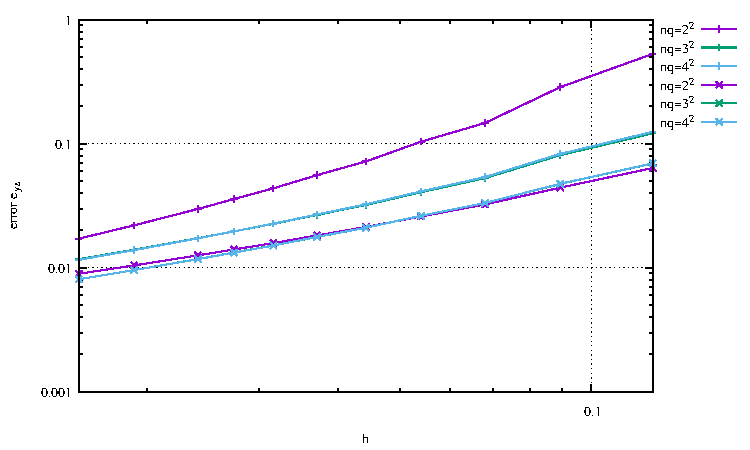
\includegraphics[width=5cm]{python_codes/fieldstone_75/results/burst/errors_eyz}\\
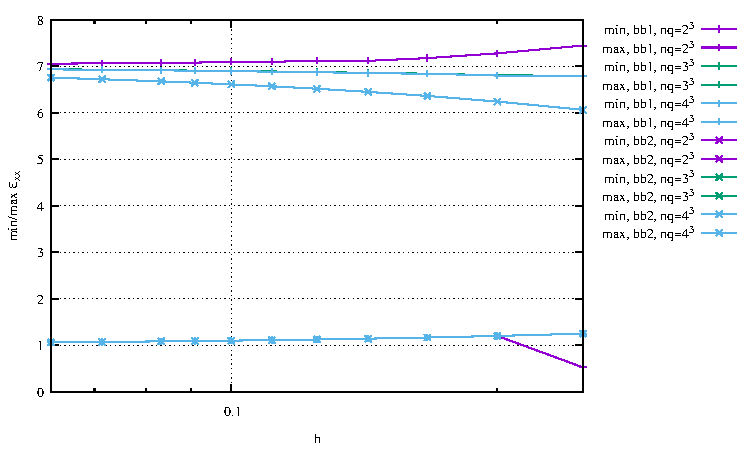
\includegraphics[width=5cm]{python_codes/fieldstone_75/results/burst/exx_stats.pdf}
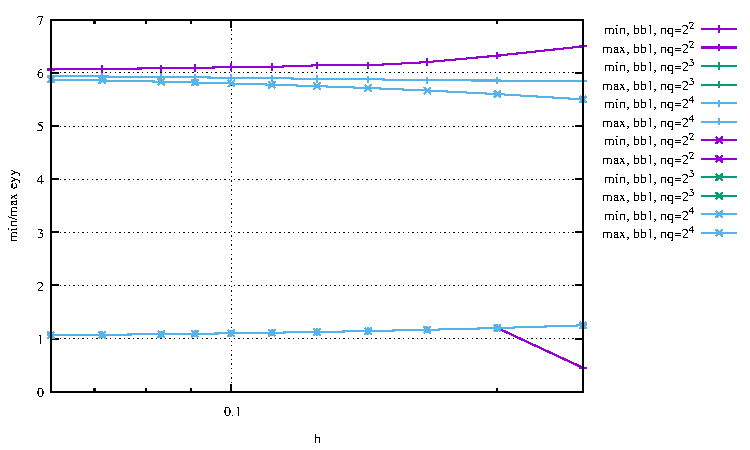
\includegraphics[width=5cm]{python_codes/fieldstone_75/results/burst/eyy_stats.pdf}
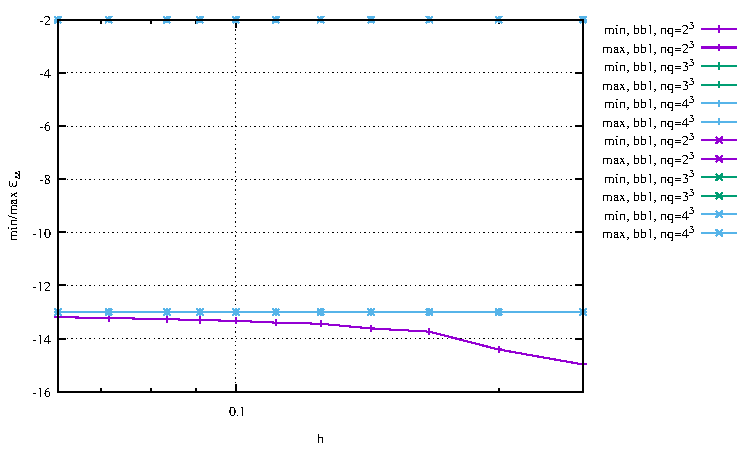
\includegraphics[width=5cm]{python_codes/fieldstone_75/results/burst/ezz_stats.pdf}\\
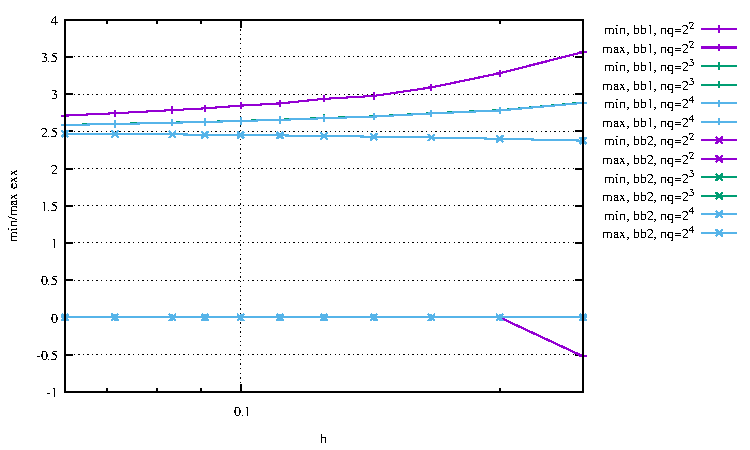
\includegraphics[width=5cm]{python_codes/fieldstone_75/results/burst/exy_stats.pdf}
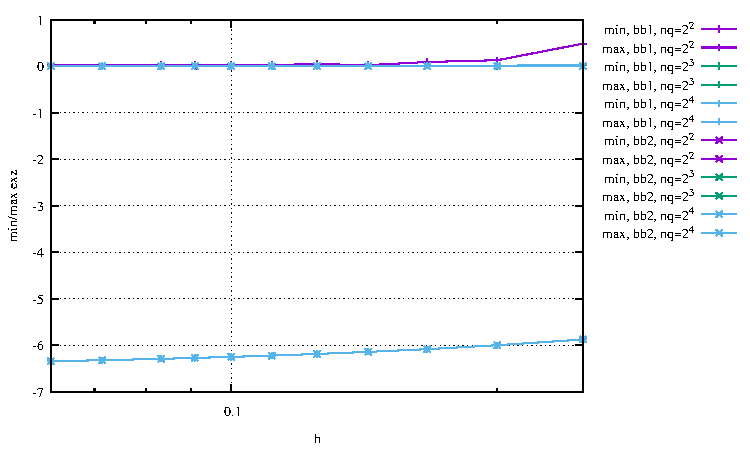
\includegraphics[width=5cm]{python_codes/fieldstone_75/results/burst/exz_stats.pdf}
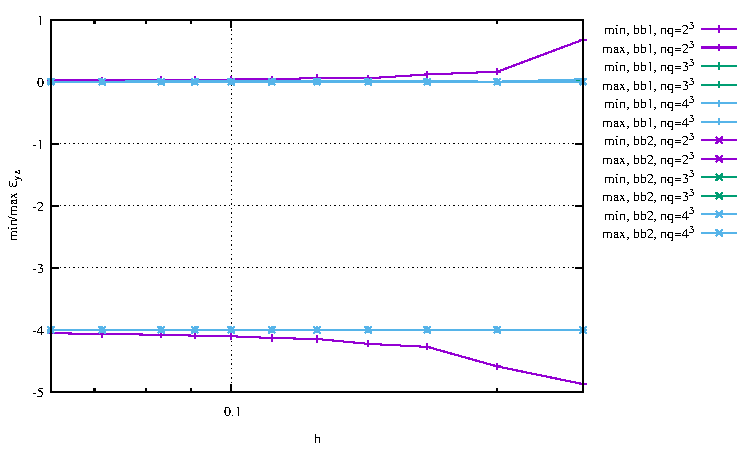
\includegraphics[width=5cm]{python_codes/fieldstone_75/results/burst/eyz_stats.pdf}\\
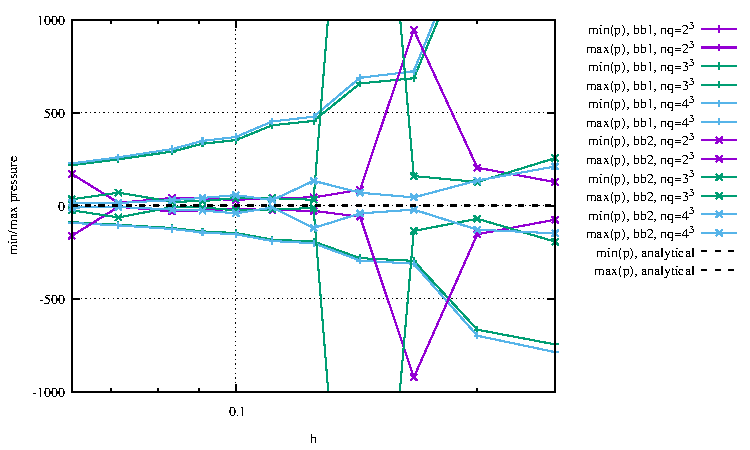
\includegraphics[width=10cm]{python_codes/fieldstone_75/results/burst/p_stats.pdf}
%{\captionfont opla  }
\end{center}

\begin{center}
a)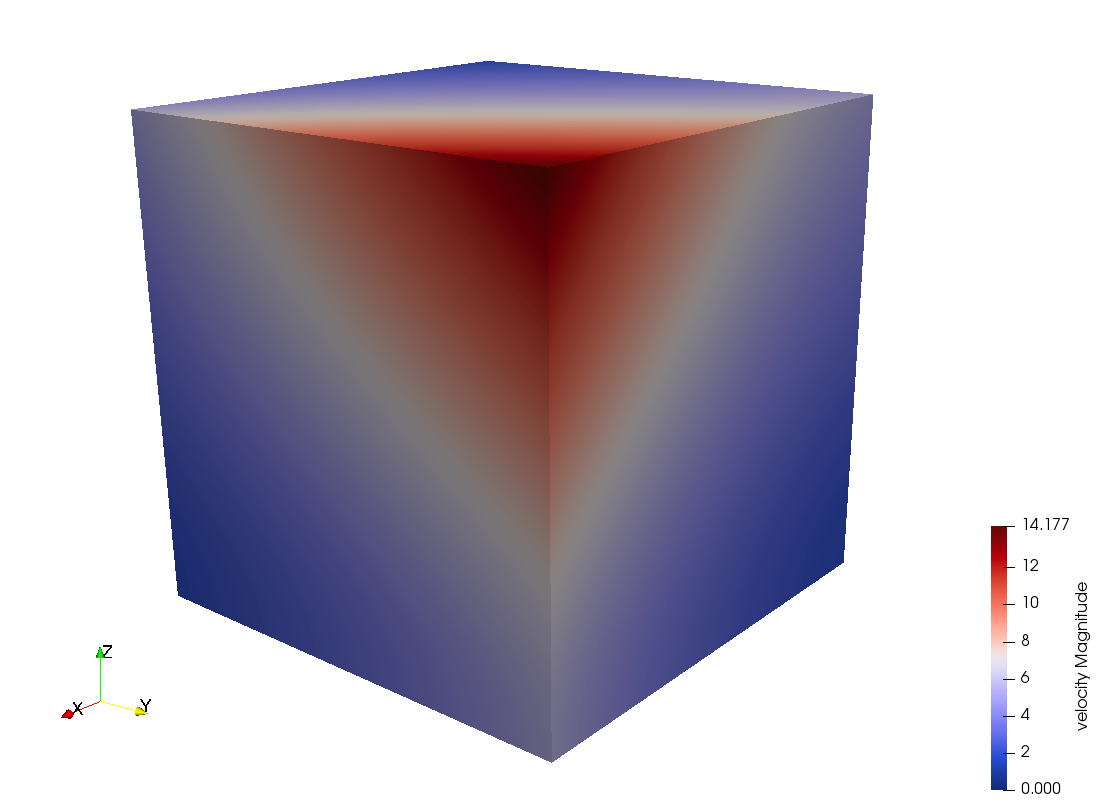
\includegraphics[width=4.5cm]{python_codes/fieldstone_75/results/burst/vel.png}
b)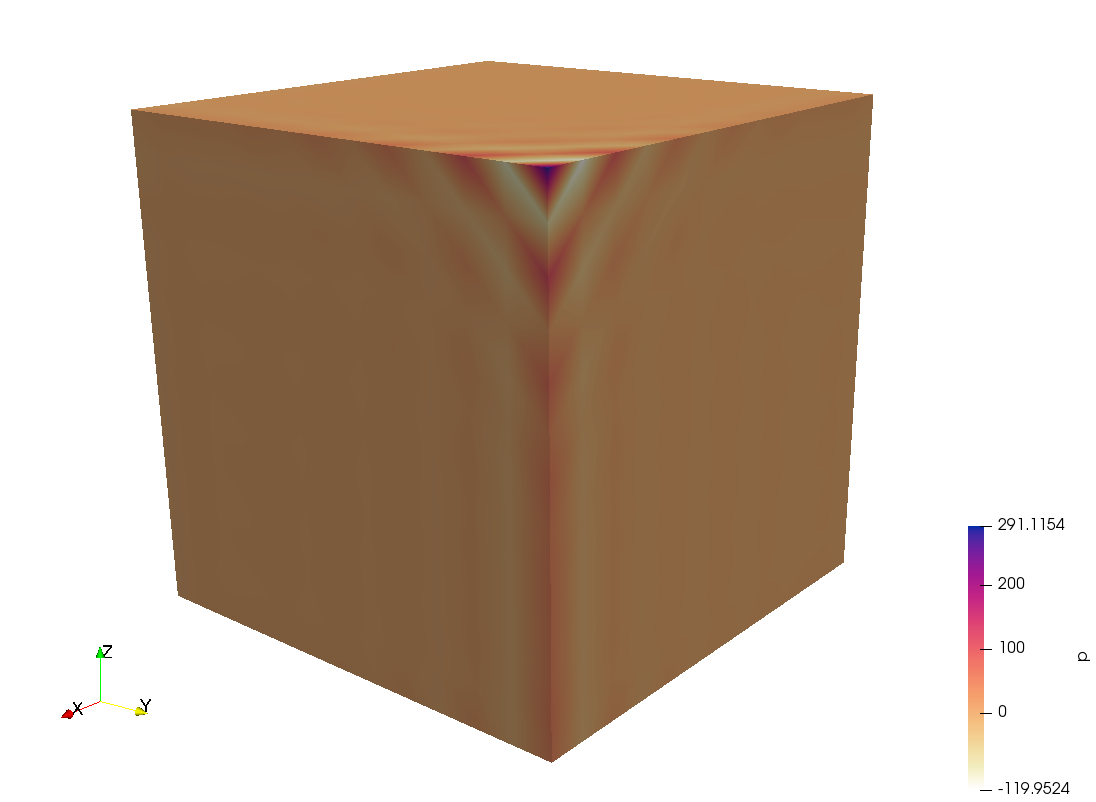
\includegraphics[width=4.5cm]{python_codes/fieldstone_75/results/burst/p_b1}
c)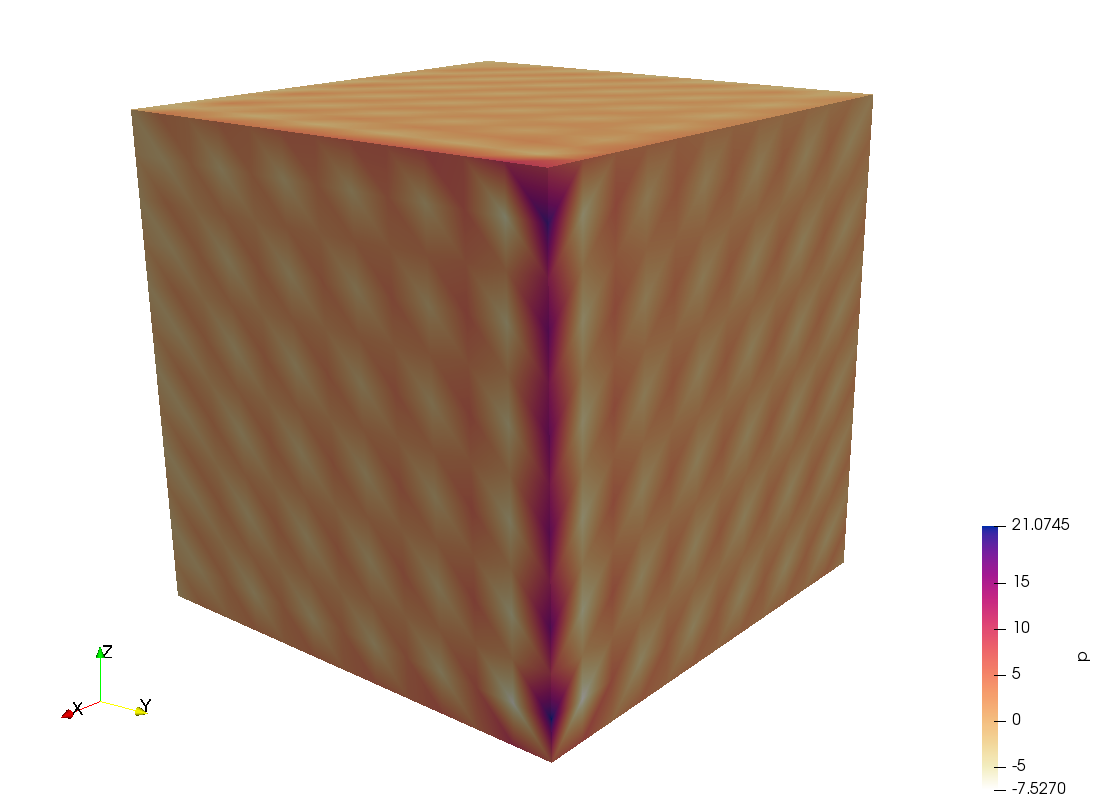
\includegraphics[width=4.5cm]{python_codes/fieldstone_75/results/burst/p_b2}\\
{\captionfont a) velocity field; b) pressure field obtained with bubble 1;
c) pressure field obtained with bubble 2. Resolution 12x12x12.}
\end{center}

We see that in this case the bubble \#2 is way worse than bubble \#1. However both 
yield very bad pressure fields, although the pressure min/max value seem to converge 
towards the analytical values for bubble \#1. However, given how insanely slow Python 
is, I cannot test this with resolutions higher than 20x20x20...
Also I need to implement a better solver. Take it from stone 16. 


%...........................................................................
\paragraph{The generic mms3D} It is defined in Section~\ref{ss:mms3Dgen}. 
Python file is {\tt stone\_mms3D.py}

\begin{eqnarray}
u(x,y,z) &=& x(1-x)(1-2y)(1-2z)\\
v(x,y,z) &=& (1-2x) y(1-y) (1-2z) \\
w(x,y,z) &=& -2(1-2x)(1-2y)z(1-z) \\
p(x,y,z) &=& (2x-1)(2y-1)(2z-1)
\end{eqnarray}

\begin{center}
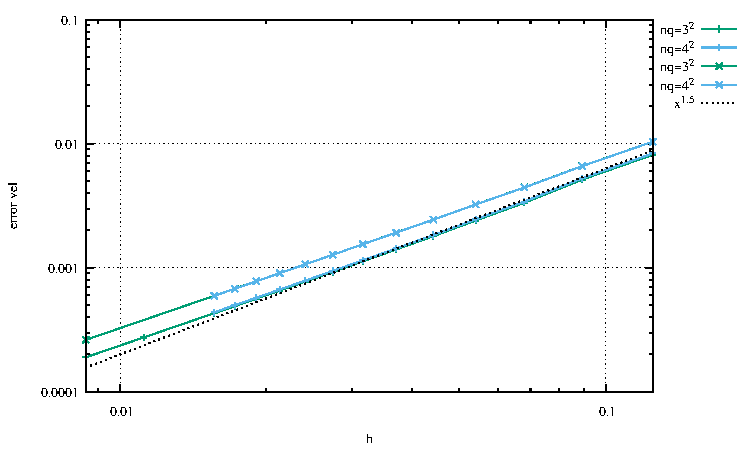
\includegraphics[width=5cm]{python_codes/fieldstone_75/results/mms3D/errors_v.pdf}
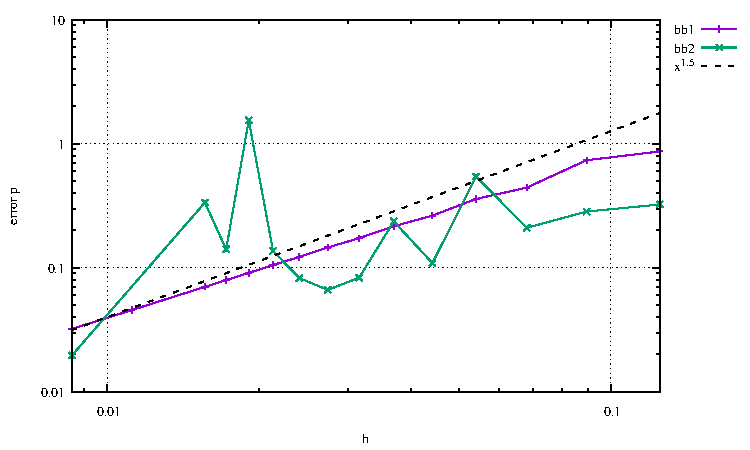
\includegraphics[width=5cm]{python_codes/fieldstone_75/results/mms3D/errors_p.pdf}
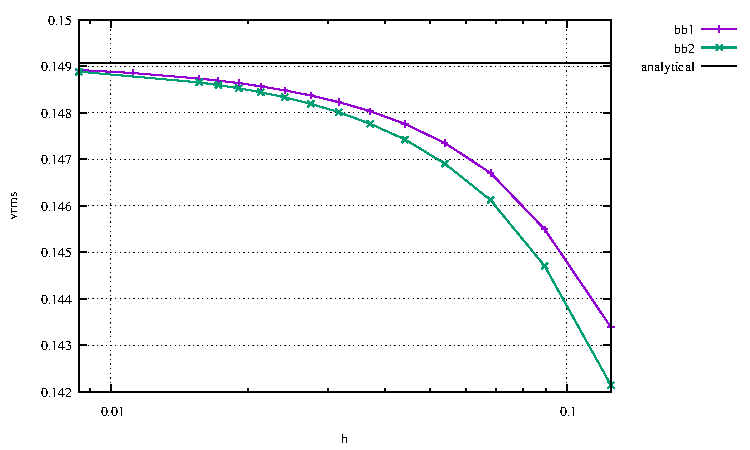
\includegraphics[width=5cm]{python_codes/fieldstone_75/results/mms3D/vrms.pdf}\\
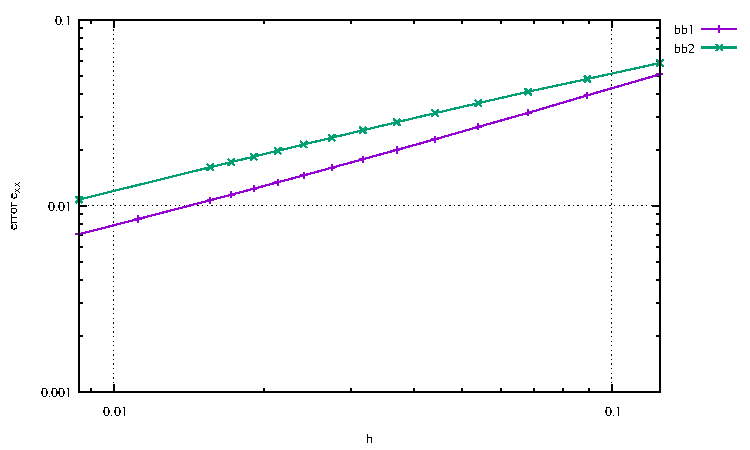
\includegraphics[width=5cm]{python_codes/fieldstone_75/results/mms3D/errors_exx}
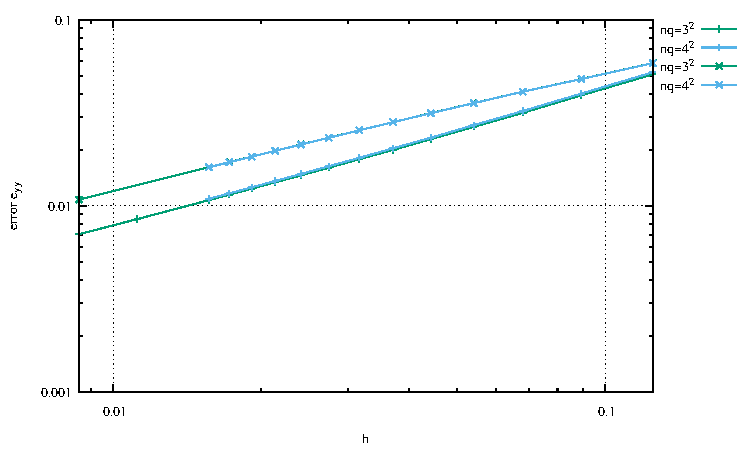
\includegraphics[width=5cm]{python_codes/fieldstone_75/results/mms3D/errors_eyy}
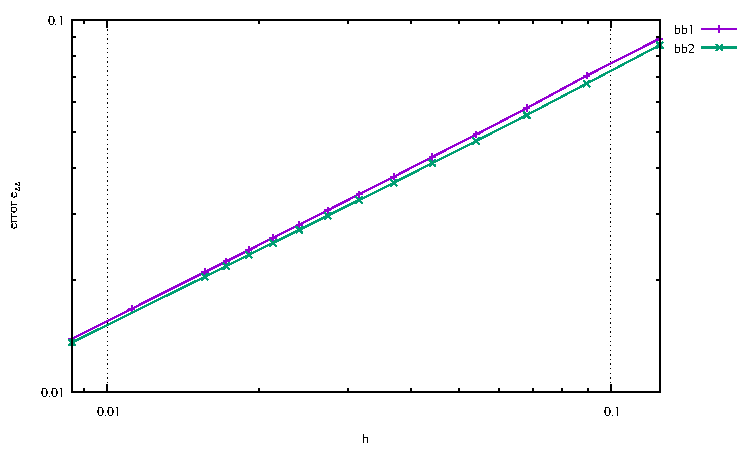
\includegraphics[width=5cm]{python_codes/fieldstone_75/results/mms3D/errors_ezz}\\
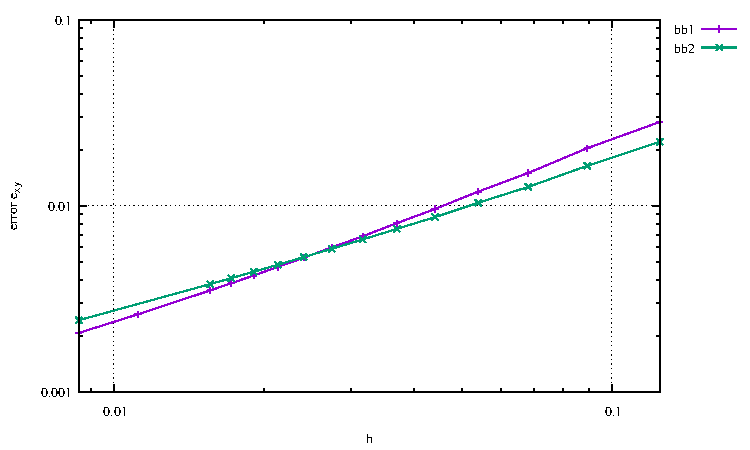
\includegraphics[width=5cm]{python_codes/fieldstone_75/results/mms3D/errors_exy}
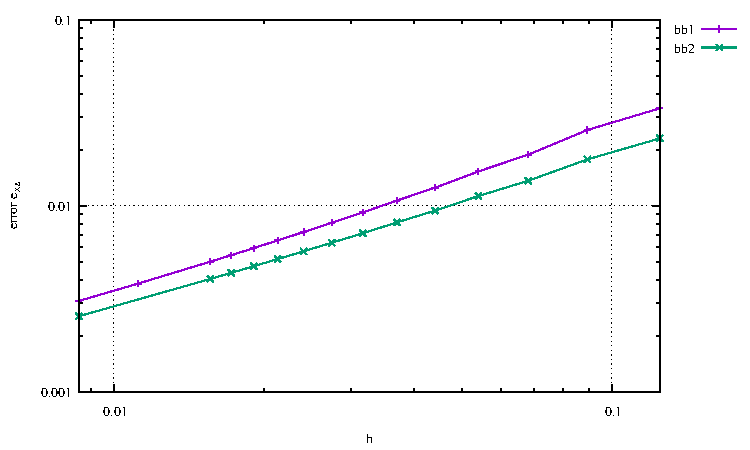
\includegraphics[width=5cm]{python_codes/fieldstone_75/results/mms3D/errors_exz}
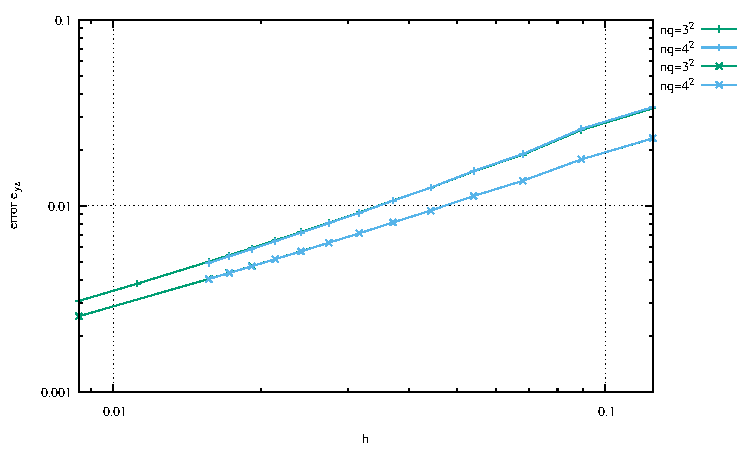
\includegraphics[width=5cm]{python_codes/fieldstone_75/results/mms3D/errors_eyz}\\
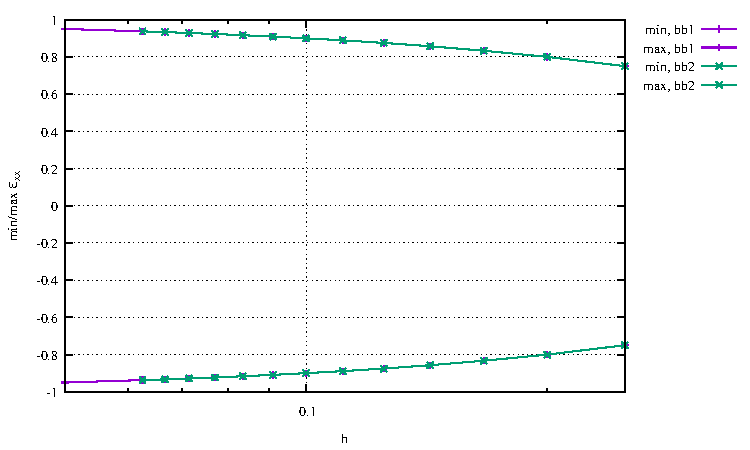
\includegraphics[width=5cm]{python_codes/fieldstone_75/results/mms3D/exx_stats.pdf}
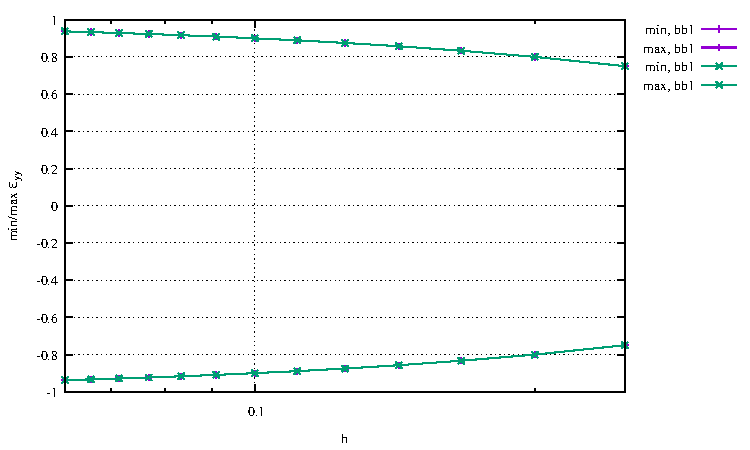
\includegraphics[width=5cm]{python_codes/fieldstone_75/results/mms3D/eyy_stats.pdf}
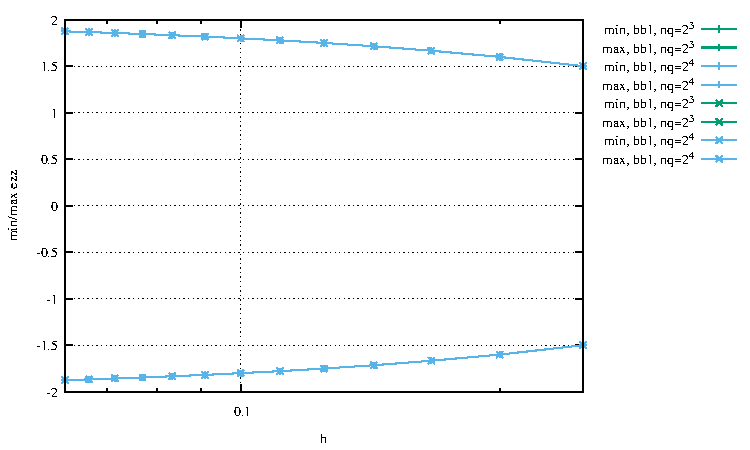
\includegraphics[width=5cm]{python_codes/fieldstone_75/results/mms3D/ezz_stats.pdf}\\
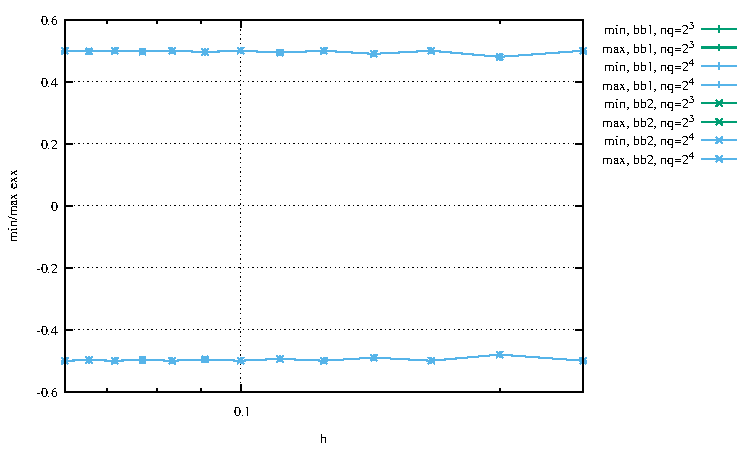
\includegraphics[width=5cm]{python_codes/fieldstone_75/results/mms3D/exy_stats.pdf}
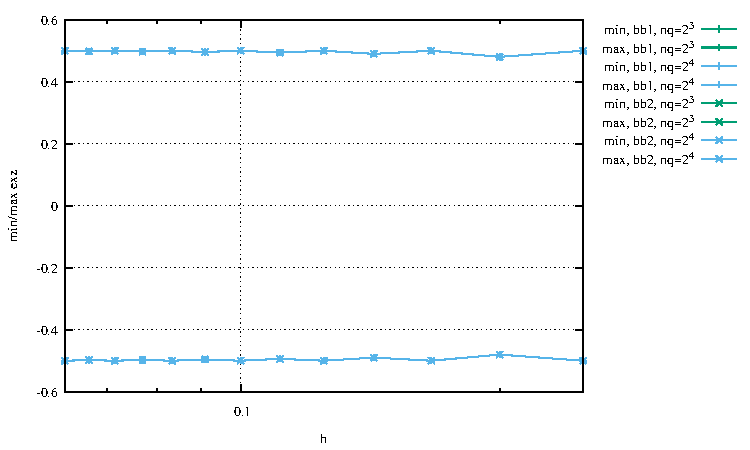
\includegraphics[width=5cm]{python_codes/fieldstone_75/results/mms3D/exz_stats.pdf}
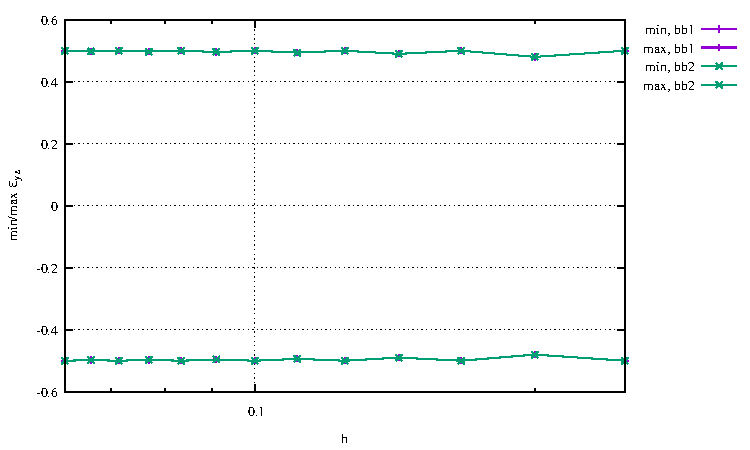
\includegraphics[width=5cm]{python_codes/fieldstone_75/results/mms3D/eyz_stats.pdf}\\
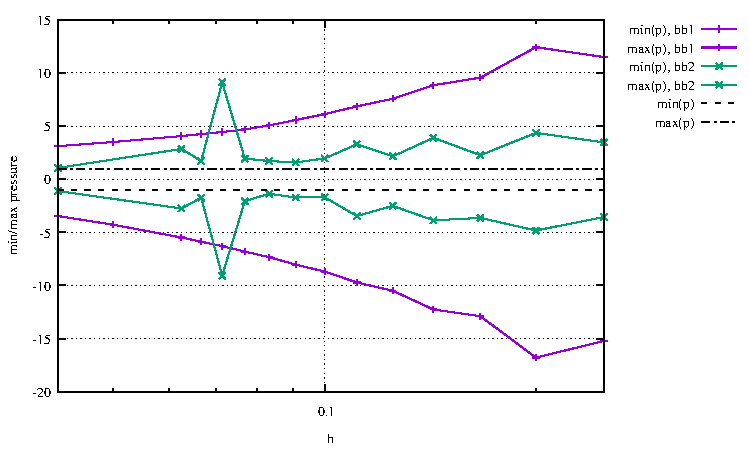
\includegraphics[width=10cm]{python_codes/fieldstone_75/results/mms3D/p_stats.pdf}
%{\captionfont opla  }
\end{center}


\begin{center}
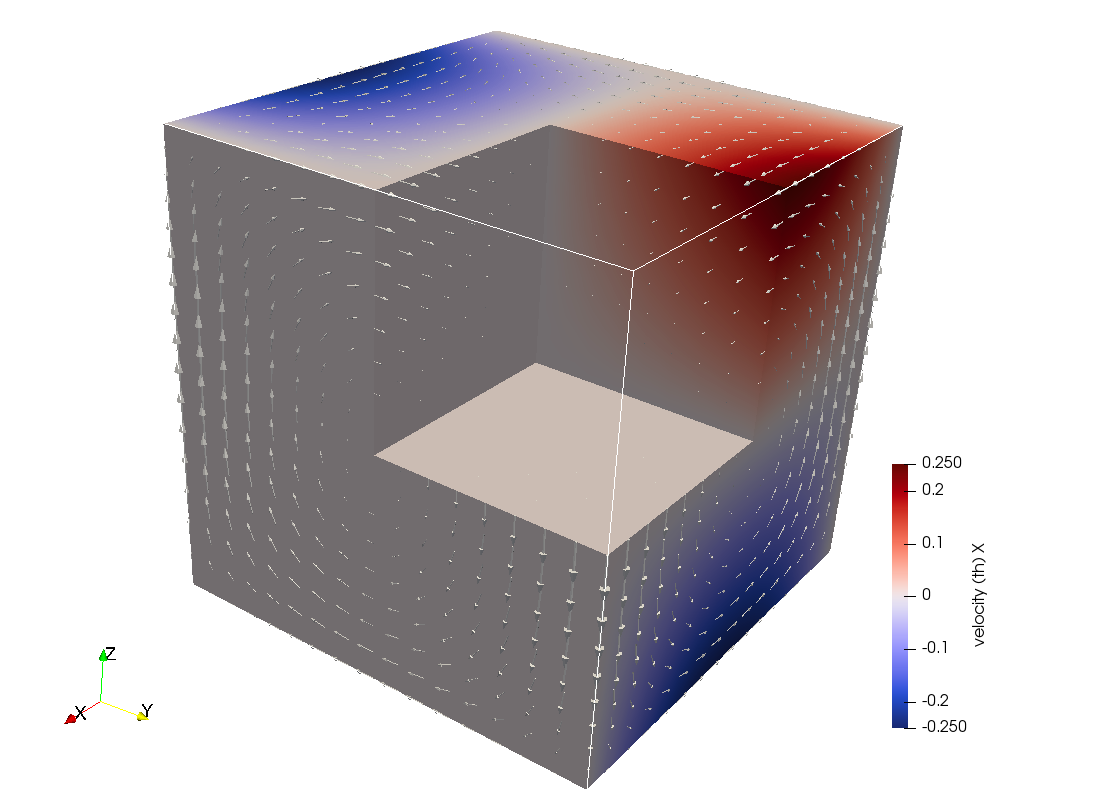
\includegraphics[width=5cm]{python_codes/fieldstone_75/results/mms3D/u}
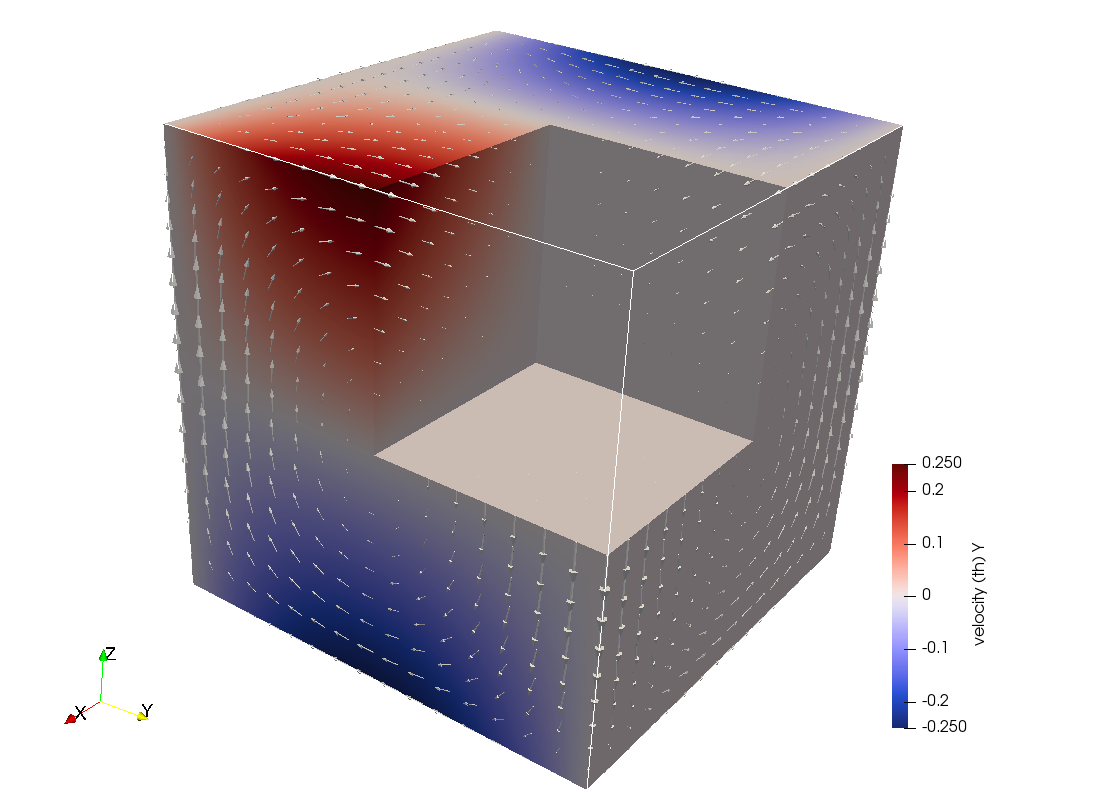
\includegraphics[width=5cm]{python_codes/fieldstone_75/results/mms3D/v}
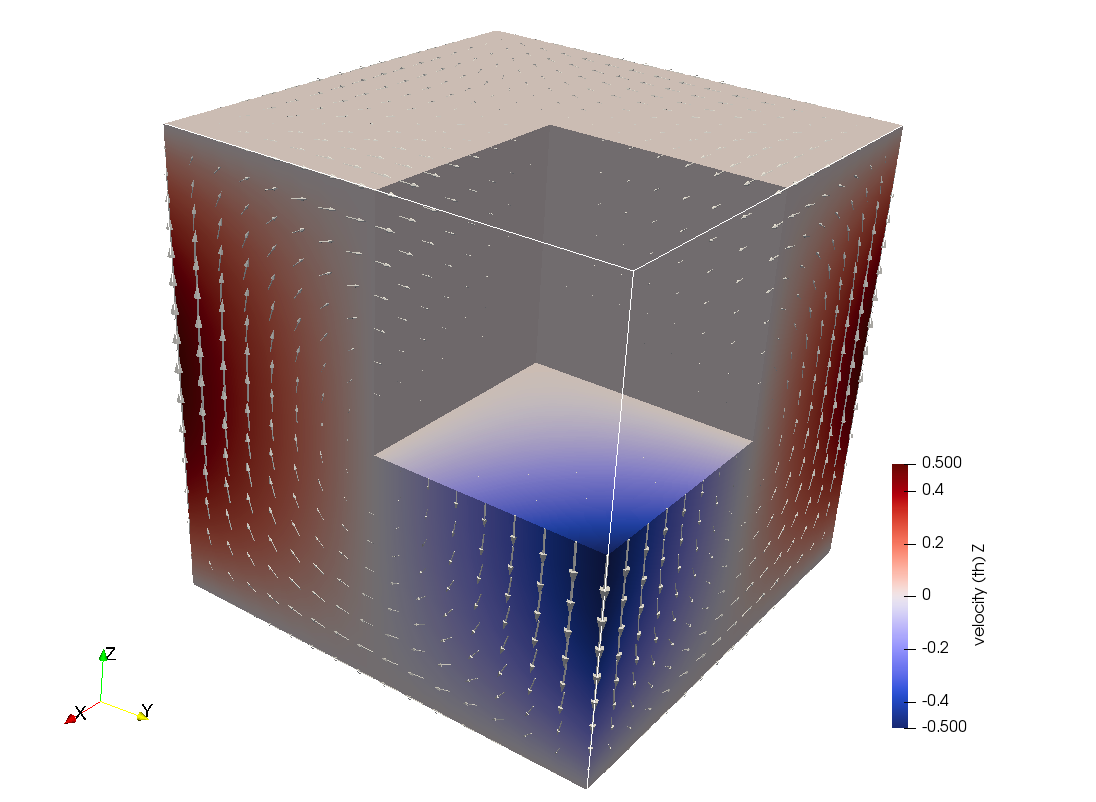
\includegraphics[width=5cm]{python_codes/fieldstone_75/results/mms3D/w}\\
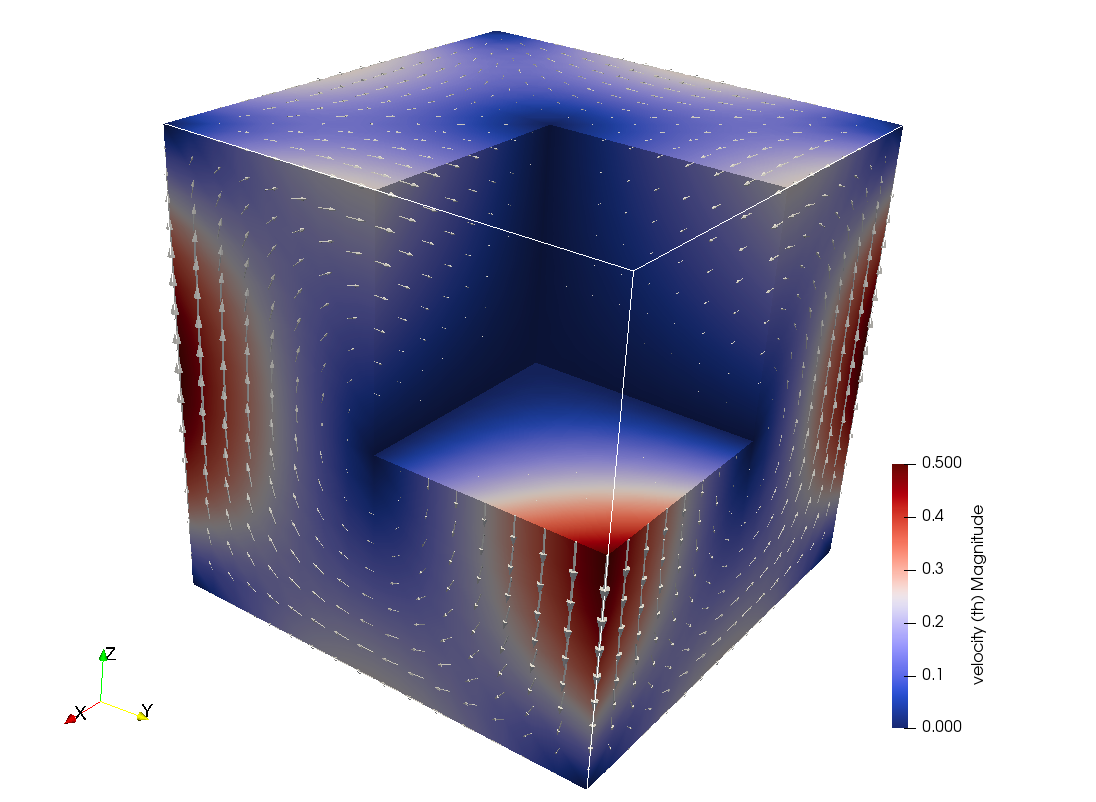
\includegraphics[width=7cm]{python_codes/fieldstone_75/results/mms3D/vel}
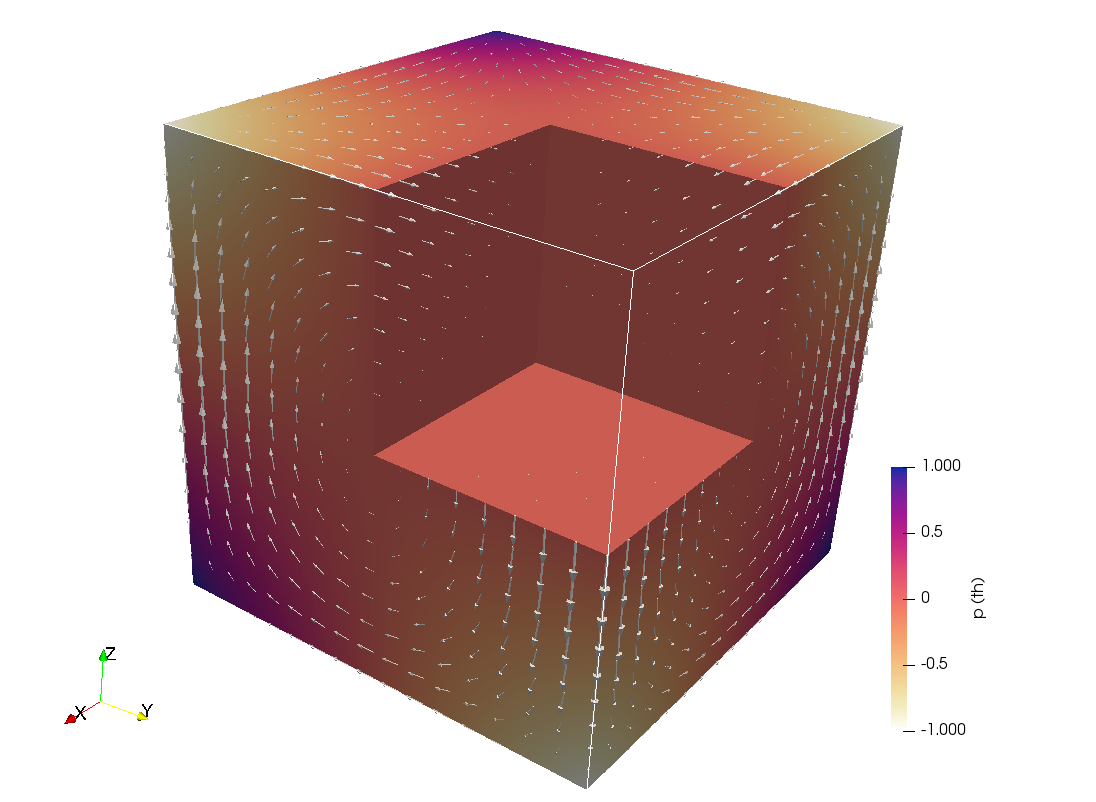
\includegraphics[width=7cm]{python_codes/fieldstone_75/results/mms3D/p}\\
{\captionfont Velocity and pressure fields (analytical values)}
\end{center}

\begin{center}
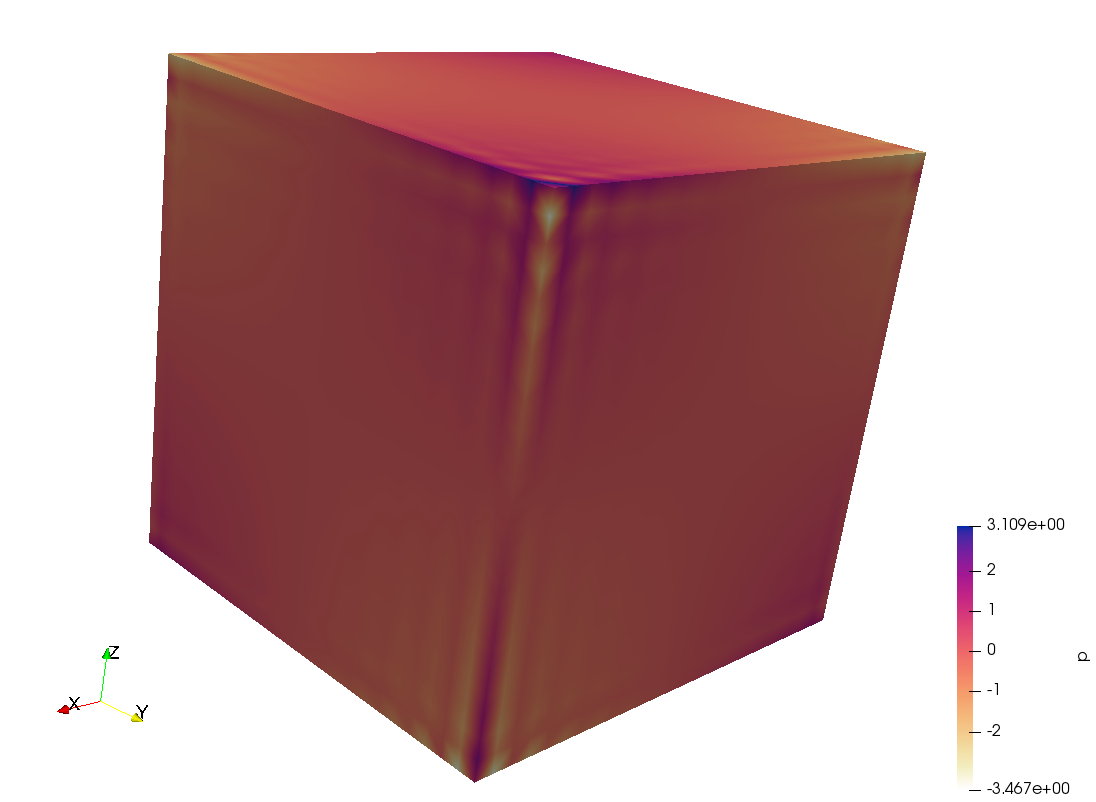
\includegraphics[width=7cm]{python_codes/fieldstone_75/results/mms3D/p_b1}
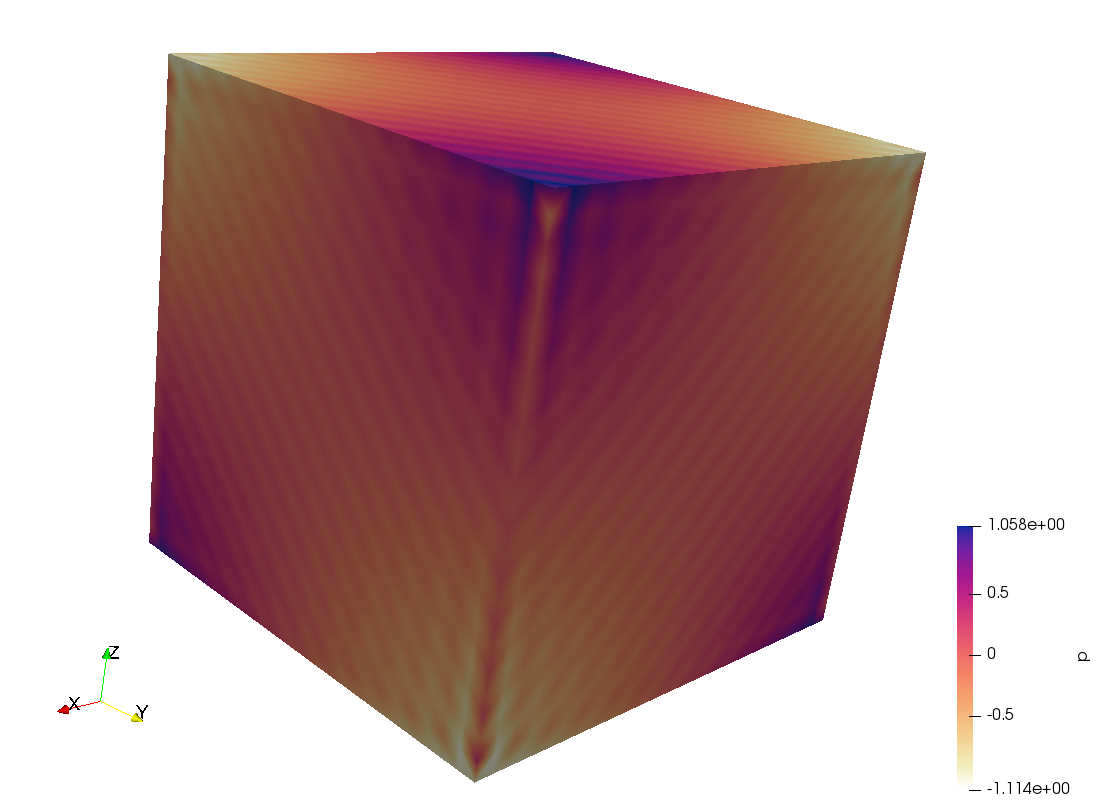
\includegraphics[width=7cm]{python_codes/fieldstone_75/results/mms3D/p_b2}\\
{\captionfont Pressure. Left: bubble \#1, Right: bubble \#2.}
\end{center}

It would be interesting to see such results for a 32x32x32 resolution... 

